\begin{abstract}

何かしらの処理を実行するとき、コンピュータが得意なことはコンピュータに、人は人にしかできないことや人がやるべきことに集中すべきだ。何かしらの処理を実行するとき、コンピュータが得意なことはコンピュータに、人は人にしかできないことや人がやるべきことに集中すべきだ。何かしらの処理を実行するとき、コンピュータが得意なことはコンピュータに、人は人にしかできないことや人がやるべきことに集中すべきだ。何かしらの処理を実行するとき、コンピュータが得意なことはコンピュータに、人は人にしかできないことや人がやるべきことに集中すべきだ。何かしらの処理を実行するとき、コンピュータが得意なことはコンピュータに、人は人にしかできないことや人がやるべきことに集中すべきだ。何かしらの処理を実行するとき、コンピュータが得意なことはコンピュータに、人は人にしかできないことや人がやるべきことに集中すべきだ。

\end{abstract}

\maketitle

\section{はじめに}\label{ux306fux3058ux3081ux306b}

あらゆるモノ・コトがプログラムで記述されるような未来が近づいている
プログラムで処理できることは増え続けている
実世界においても、それは言えること
実世界志向インタフェースなどの研究は多くの成果を出している
Hueなどの商品によって、実際に誰でもプログラムできるようになってきている
この流れは変わらず、全世界がプログラム可能になっていくと考えられる。

一方で、コンピュータのみでは処理できないようなこともある
人の確認が必要な状況 人の意志の反映が求められる状況
人でなくてはいけないような状況
こういった問い合わせはプログラムに組み込みづらい
結果として、プログラム化・自動実行などが難しくなっている。

コンピュータの方が得意なこともあれば、人のほうが得意なこともある
何かしらの処理を実現する上で、コンピュータと人は相補的に動作していくべきである
今までは出来なかったようなことの実現

上記の状況を踏まえ、本論文では
プログラムから人へ、処理命令を送れる人力処理組み込み環境 Babascript
を提案する。 Babascript環境では、プログラムというフォーマット上において
コンピュータと人、双方への命令を同様のインタフェースで記述可能になる
特殊なプログラミング言語を導入せず、既存の言語上において実現可能

コンピュータはプログラムという手順書を実行する
人も、常日頃から手順書に基づいて行動している ex: マニュアル、レシピ
手順書のフォーマットが異なるだけで、処理内容が記述された手順書を参照していることには変わらない
つまり、手順書のフォーマットは同一にすることも可能である。

\section{Babascript}\label{babascript}

Babascript環境では、プログラムに人を組み込めるようにするために、関数呼び出しによって人に命令を送れる仕組みを持つ。
通常のプログラムでは、関数に引数を与え、実行することで、その関数の名に適した処理が行われた後、返り値として処理結果を得ることが出来る。
Babascriptでは、同様に関数呼び出しし、処理を人に実行させ、返り値を処理結果として返す。
プログラム上においては、両者は同じ関数呼び出しだが、その実行主体を人間にすることによって、プログラム内における人力処理の組み込みを実現する。
である。

このような仕組みを実現するために、人への命令構文を持ったDSL Babascript
と、命令に対して返り値を返すためのクライアントライブラリ
BabascriptClientと、クライアントライブラリを組み込んだWebアプリケーションを開発した、
また、プラグイン機構によってその機能を拡張可能にした。

\subsection{Script}\label{script}

Babascriptは、関数呼び出しによって人に対して処理命令を送れるオブジェクト(以下、人オブジェクト)を宣言可能にするDSLだ。
人オブジェクトにおいて定義されていない全てのメソッドが人への命令として解釈される。
また、命令に対して人からの返り値を得ると、実行メソッドの引数で指定したコールバック関数を実行する。

\subsubsection{人オブジェクトの宣言と処理命令構文}\label{ux4ebaux30aaux30d6ux30b8ux30a7ux30afux30c8ux306eux5ba3ux8a00ux3068ux51e6ux7406ux547dux4ee4ux69cbux6587}

図1のようなプログラムによって、人への処理命令を送ることができる。

\begin{verbatim}
baba = new Baba.Script "baba"
baba.ほげふが (task) ->
  console.log 'hoge'
\end{verbatim}

人オブジェクトは宣言時にIDを指定することによって、誰に対して処理命令を配信するかを決定する。
実行された処理命令は、指定したIDを監視するクライアントライブラリにのみ配信される。
この際、指定したIDを監視するクライアントが複数人、つまり、グループを形成していた場合、人への命令構文を実行時に他のタスクを実行していないクライアントへと順番にタスクが配信される。

人への処理命令構文は、実行されるとメソッド名と引数を元にしたjsonオブジェクトへと変換され、このjsonオブジェクトが処理命令のデータとしてクライアントライブラリに配信される。

人への処理命令構文の第一引数には基本的な処理情報に加えてクライアント側に送信するオプション情報を指定する。
第二引数には、人から処理命令に対する返り値が得られた際に実行するコールバック関数を指定する。
コールバック関数実行時には、その引数に返り値と関連した情報を格納したオブジェクトが与えられる。

オブジェクトに定義されていない全ての関数は人への処理命令構文として解釈される。
この機能はmethodmissingという、定義されていないメソッドが実行された際にその処理を記述しておく仕組みによって実現する。

\subsubsection{オプション情報の付加}\label{ux30aaux30d7ux30b7ux30e7ux30f3ux60c5ux5831ux306eux4ed8ux52a0}

人への処理命令構文の第一引数に与えるオプション情報には、返り値の型指定などの情報が考えられる。
返り値としてあらゆる型を想定したプログラムを記述することは難しい。
例えばBoolean型で返してほしい、といった時には図2のようなプログラムが考えられる。

\begin{verbatim}
baba.ほげふが {format: 'boolean'}, (task) ->
    console.log task
\end{verbatim}

他にも、指定したリストの中から値を選択してほしい、といった命令の場合は、そのリストをオプション情報として付加することが考えられる。

特別なオプション情報として、broadcastオプションが存在する。
broadcast機能は、指定したIDを監視する全てのクライアントへとタスクを配信し、指定した数の返り値を得られると処理を終了し、コールバック関数を実行するといったものだ。

\subsection{Client}\label{client}

Babascript
Clientは、Babascriptからの命令受信と処理結果の送信機能を実現するクライアントライブラリだ。
命令受信のイベントに対してコールバック関数を指定することで、処理命令を受け取ることができる。
基本的な利用方法は、図3に示す。

\begin{verbatim}
client = new BabascriptClient "baba"
client.on "get_task", (task) ->
    # タスク受信後の動作を記述する
\end{verbatim}

クライアントオブジェクトの宣言時、IDを指定することによって、IDに対して処理命令が発行された際にタスクを受信することができる。
また、クライアントオブジェクトが持つ ``returnValue''
メソッドを利用することで、返り値を命令発行元に返すことができる。

このClientライブラリを組み込み、ユーザに提示するためのWebアプリケーションを実装した。
タスク情報において型指定をすることによって、ユーザに提示するUIを変化させ、型に合った返り値を選択できるようにしている。
例えば、Boolean型を指定していた場合、ユーザには true ボタンと false
ボタンが提示され、どちらかを押すと、その結果が返り値としてプログラムに返される。
また、String型を指定すれば、文字列の入力フォームとSubmitボタンが表示される。
スマートフォンに最適化したWebアプリケーションとして実装しており、様々な場面において利用可能であり、実世界におけるタスクを処理しながらでも十分に利用可能であると言える。

クライアントライブラリは、UIと完全に分離した実装となっており、かつ利用方もシンプルだ。
上記のWebアプリケーションだけでなく、新規/既存問わず、様々なアプリケーションに組み込むことができる。

\subsection{Plugin}\label{plugin}

Pluginは、Babascript及びBabascript
Clientに組み込むことのできるプラグイン機構だ。
Babascript及びBabascriptClientが発行するイベントとデータを受け取ることができる。
以下のようなイベントを受け取り、その都度処理を実行させることができる。

\begin{itemize}
\itemsep1pt\parskip0pt\parsep0pt
\item
  init(プラグイン読み込み時)
\item
  connect(ネットワーク接続時)
\item
  send(タスクの送信時)
\item
  receive(タスクの受信時)
\end{itemize}

以下のようなプログラムによって、プラグインを読み込むことができる

\begin{verbatim}
baba = new Babascript("baba")
baba.use(new Logger())
\end{verbatim}

具体的には、以下のようなプラグインの実装が挙げられる。

\begin{itemize}
\itemsep1pt\parskip0pt\parsep0pt
\item
  ログコレクター
\item
  データ同期
\item
  ユーザ管理
\end{itemize}

\subsection{通信と分散処理}\label{ux901aux4fe1ux3068ux5206ux6563ux51e6ux7406}

scriptとclientのタスク送受信と分散配信のために、node-linda\cite{linda}を利用した。
Websocketによる通信が行われ、リアルタイムにタスクの送受信が行われている。
script,
client共に、このnode-lindaに接続するためのライブラリを組み込んでいる。

scriptは、プログラム実行時にnode-lindaサーバに接続し、人への命令構文を実行するごとに、タスクをnode-lindaサーバに書き込む。
書き込み終了後、そのタスクと同じIDを持った返り値タスクが書き込まれるまで、node-lindaサーバの監視を行う。

clientは、プログラム起動中は常にnode-lindaサーバに接続し、指定されたIDを監視する。

\subsection{実装}\label{ux5b9fux88c5}

上記システムは全てJavascriptで実装した。 Babascript
はNode.js上で動作し、 Babascript
ClientはNode.jsとWebブラウザ上で動作する。
全体図は図\ref{system}のとおりだ。

\begin{figure}[h]
  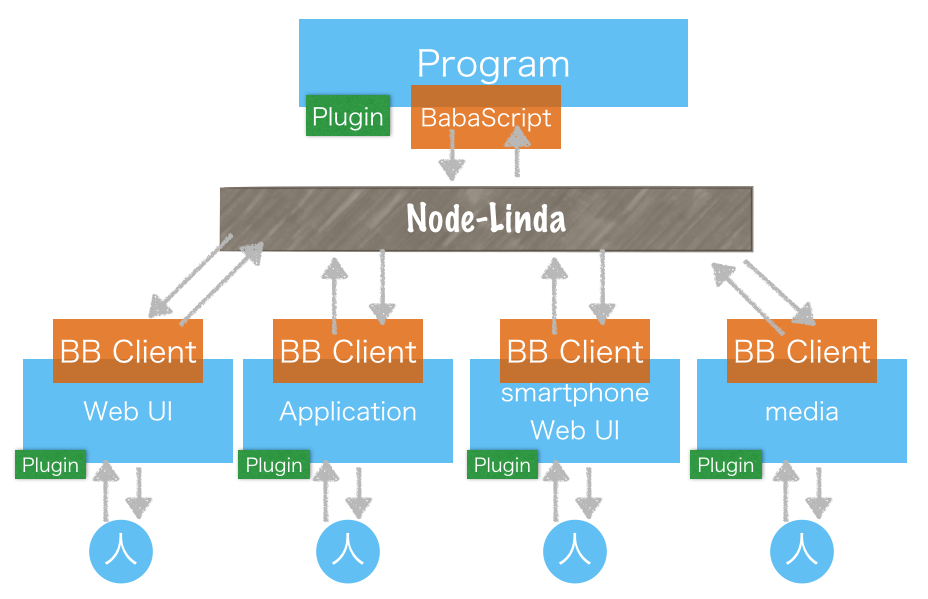
\includegraphics[width=220px]{./images/system.png}
  \caption{システム全体図}  
  \label{system}
\end{figure}

\subsubsection{タスク情報の構成}\label{ux30bfux30b9ux30afux60c5ux5831ux306eux69cbux6210}

人への処理命令構文は実行によってタスク情報を生成する。
このタスク情報は、以下のようなjsonオブジェクトとなる。

\begin{verbatim}
task = {
  "name": "baba", # 命令配信先ID
  "type": "eval", # 配信タイプ
  "key": "パン買ってこい", # 処理命令の内容    
  "cid": "'1409227153_0.8690411776769906'", 
  # タスクID
  "option": {
    "format": "boolean",
  }
  # オプション情報
}
\end{verbatim}

\subsubsection{実行結果の返し方}\label{ux5b9fux884cux7d50ux679cux306eux8fd4ux3057ux65b9}

人への命令構文に対する返り値が、適切に返り値として戻されるようにするために、命令ごとにユニークなIDを生成している。
ユニークIDは、8桁のランダムな数値と人への命令構文実行時のUnixTimeを結合した文字列である。
このユニークIDを伴った返り値が戻ってくるか、指定したタイムアウト時間に到達するか、タスクキャンセルをするまでBabascriptは返事を待ち続ける。

\subsection{サンプルプログラム}\label{ux30b5ux30f3ux30d7ux30ebux30d7ux30edux30b0ux30e9ux30e0}

\section{応用例}\label{ux5fdcux7528ux4f8b}

以下のような応用が考えられる。

\begin{itemize}
  \item 人の行動をプログラミングする
  \item 実世界をテストする
  \item あれ
\end{itemize}

\subsection{人の行動をプログラミングする}\label{ux4ebaux306eux884cux52d5ux3092ux30d7ux30edux30b0ux30e9ux30dfux30f3ux30b0ux3059ux308b}

仕事や役割などは、コンピュータと人の両方の作業で成り立つ
人が代替可能になる 人が状態を管理する必要がなくなる

\subsection{実世界をテストする}\label{ux5b9fux4e16ux754cux3092ux30c6ux30b9ux30c8ux3059ux308b}

\section{議論}\label{ux8b70ux8ad6}

\subsection{一処理単位としての人}\label{ux4e00ux51e6ux7406ux5358ux4f4dux3068ux3057ux3066ux306eux4eba}

本研究では、人はコンピュータ等と同じ、処理を命令され実行するノードとして扱われると思われる。
けど、これは人が人にしかやれないようなことや、人がやるべきことだけに集中できるような環境を構築するためのもの。
人から見れば、条件判断を出来るだけプログラムとして記述できるほうが、処理実行もしやすい。

\subsection{タスク実行の遅延と実行保障性}\label{ux30bfux30b9ux30afux5b9fux884cux306eux9045ux5ef6ux3068ux5b9fux884cux4fddux969cux6027}

Babascriptによってタスク実行を依頼しても、人がすぐにタスクを実行し値を返すことを完全に保証することはできない。
タスク受信端末を見ていない、受信しても実行できないといった状況の場合、すぐに値を返すことはできない。
こういった際、Babascriptによる処理がボトルネックとなる可能性がある。

また、労働関係にあるなど、タスク実行に強制力がある場合は、タスク実行が確実に行われると考えられるが、強制力がない場合はそもそもタスク受信を無視するといったことも考えられる。
タスク実行に強制力がない場合は、金銭などのインセンティブを与えるといった手段によって、実行保障性を確保するといったことが考えられる。

\subsection{命令内容の粒度}\label{ux547dux4ee4ux5185ux5bb9ux306eux7c92ux5ea6}

Babascriptでは、タスクの文面の記述には制限がないため、自由となっている。
この文面は、適切な抽象度の文面に設計しなくてはならない。
抽象度が高すぎる命令は、あいまいな表記となり、タスク実行者にとって理解しづらい文面となり得る。
その結果、想定外の処理が実行され、意図しない結果を招く恐れがある。
抽象度が低すぎる命令は、全体の処理内容にもよるが、プログラム自体が冗長となり得る。
プログラムとタスク実行者の間のやりとりが増え、通信や待機時間などがボトルネックとなる可能性がある。
また、タスク実行者にとっても、やりとりが増えることで負担増になると考えられる。

\subsection{同時の複数命令}\label{ux540cux6642ux306eux8907ux6570ux547dux4ee4}

複数のプログラムから同時に一人のタスク実行者へとタスクが配信される可能性がある。
この際、異なるコンテキストにある命令が交互に配信され、タスク実行に大きな障害をもたらす可能性がある。
例えば、料理プログラムと掃除プログラムが同時に実行された場合、鍋で煮ている途中で「洗剤を投入しろ」などといった命令が配信されることが考えられる。

この問題は、全てのBabascriptプログラム中において、一人のタスク実行者は一つのプログラムからのみ、連続してタスクを受信できるような仕組みを用意することによって、解決可能であると考えられる。
また、応用アプリケーションでの実装になるが、コンテキストを明示し、どの処理系におけるタスクなのかをタスク実行者に示すといった手段によっても解決可能である。

\section{関連研究}\label{ux95a2ux9023ux7814ux7a76}

計算機では処理が難しいようなタスクを解決するために、人を計算資源として利用する手法はヒューマンコンピュテーション\cite{HumanComputation}と呼ばれ、様々な研究が行われている。
インターネットを介して不特定多数の群衆にタスクを実行させるクラウドソーシングと組み合わせた研究事例も多く存在する。
クラウドソーシングのプラットフォームとしては、Amazon Mechanical
Turk\cite{mechanicalturk}が存在する。 Barowy
らは、CrowdProgrammingという概念を提唱し、プログラミング言語内においてクラウドソーシングによる計算とコンピュータによる計算の統合を実現した\cite{automan}。
Franklin
らは、機械だけでは答えられないようなDBへのクエリに対する応答を、クラウドソーシングを用いることで返答可能にするCrowdDBを提案している\cite{crowddb}。
Morishima
らは、人をデータソースとしてプログラムの中で利用する手法を提案している\cite{cylog}。
jabberwocky crowdforge
これらの研究では、人を計算資源やデータソースとしてシステムに組み込むことを狙っている。
本研究では、計算資源やデータソースに限らず、実世界への干渉等も対象としており、本研究はより汎用的な枠組みとなっている。
また、いずれもクラウドソーシングの利用を前提としているが、本研究は不特定多数の群衆を対象としたものではない。
家族であったり、職場の人であったりといった、特定可能な人を対象としている。

ユビキタスコンピューティングの研究分野においては、Human as
Sensorという概念も提唱されている。
PRISMは、スマートフォンを利用したセンシングプラットフォームだ\cite{prism}。
Liuらは、ソーシャルメディア上の人をセンサーとして扱ったQ\&AサービスMoboQを提案し、その検証を行った。
Human as
Sensorに類する研究では、人をセンサーとして扱うことを対象としているが、本研究ではセンサーのみを対象としていない。

Chengらは、人をモーションプラットフォームにおけるモーターやメカニカル機構の代替として利用したHaptic
Turkを提案している\cite{hapticturk}。 Haptic
Turkはゲームでの利用に特化したものだ。
本研究は、使用用途を限らない汎用的な仕組みとなっている。

加藤らは、人とロボット間でのタスク共有システム
Sharedoを提案した\cite{sharedo}。
人とロボットのタスク実行における協調は、本研究の主眼である「何かの処理を実現するとき、人とコンピュータは相補的に動作するべき」という考えと大きく類似している。

\section{おわりに}\label{ux304aux308fux308aux306b}

本論文では、人への命令構文をプログラムに付与可能なプログラミング環境Babascriptを提案した。
Babascript環境においては、プログラム上において人は、コンピュータと同じ処理ノードとして存在し、関数実行によって処理内容を受け取り、実行・値を返す存在になれる。
これによって、プログラマブルになりつつある世界において人自身もその一部になることが可能となる。

また、Babascript環境によって実現する応用例を示すことによって、人をプログラマブルにした際のメリットを示した。

今後は、議論で述べたBabascriptの問題点などを改善していく。
